\section{Aproximação de funções multidimensionais}

\subsection {Mapeamento y = f(x)}

A função escolhida para o mapeamento \(\mathbb{R}^1 \rightarrow \mathbb{R}^1\)
está representada logo abaixo. Foi definido que o intervalo de \(x\) é
\([-2\pi,2\pi]\) e que este intervalo seria discretizado a cada 0.01, a fim de
possuirmos uma quantidade grande de amostras, isto é, 1257.

\begin{equation}
y = \exp(\sin x + \cos x) + \left|x\right|
\label{eq:map1}
\end{equation}

Sem a presença de ruídos, este mapeamento produz a imagem
\ref{fig:map1_s_ruido}. A imagem \ref{fig:map1_c_ruido}, por sua vez, apresenta
o resultado da soma da função com um ruído de distribuição normal de média nula
e variância 0.64. É possível verificar que a adição do ruído prejudica
fortemente a identificação do formato inicial do mapeamento. 

\FloatBarrier
			    
	\begin{figure}[h!]
	
	\centering
	
		\begin{subfigure}{.5\textwidth} 
		  \centering
		  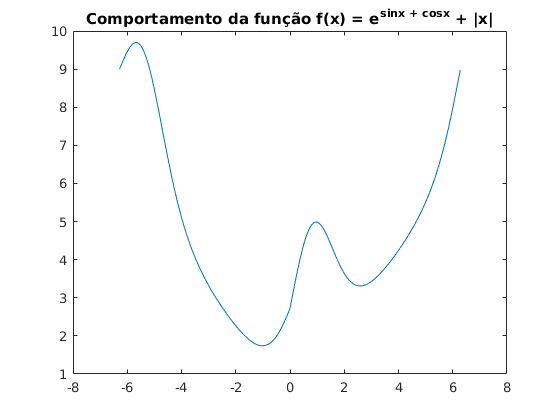
\includegraphics[width=1\linewidth]{image/sem_ruidos_y_fx}
		  \caption{\centering Mapeamento sem ruídos.} 
		  \label{fig:map1_s_ruido} 
		  
		\end{subfigure}%
		\begin{subfigure}{.5\textwidth}
		  \centering
		  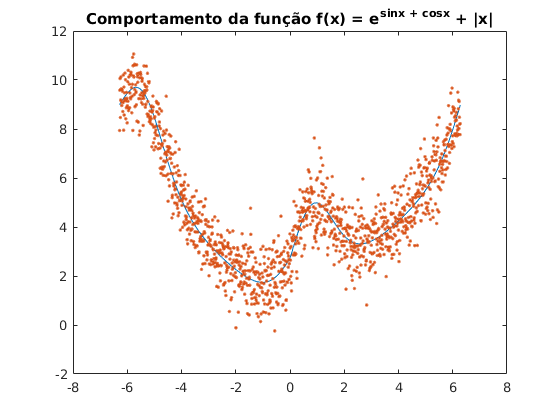
\includegraphics[width=1\linewidth]{image/com_ruidos_y_fx}
		  \caption{\centering Mapeamento com ruídos.}
		  \label{fig:map1_c_ruido} 
		\end{subfigure}
	
	
	\caption{Mapeamento da função \ref{eq:map1}.}
	\end{figure}
	
	\FloatBarrier
	
A simulação realizada no \textit{Eureqa}, primeiramente com os dados sem ruídos
e habilitando-se as funções-base exp(), sin(), cos(), abs() e as operações
básicas, forneceu os resultados contidos nas figuras
\ref{fig:map1_solucoes_s_ruido} e \ref{fig:map1_pareto_s_ruido}. A primeira
lista as soluções encontradas que mais se aproximaram dos dados amostrais.
Destaca-se que a primeira solução, cujo peso é 40, é justamente aquela que
utilizamos para produzir os dados. A segunda imagem ilustra o compromisso entre
acurácia (erro) e simplicidade (complexidade da solução). Observa-se que
inúmeras soluções apresentam erro praticamente nulo, porém existe apenas uma
cuja complexidade é mínima para este caso. Essa função trata-se da solução de
tamanho 40 que, como já foi dito, é igual à equação \ref{eq:map1}. A figura
\ref{fig:map1_best_s_ruido} apresenta um resumo da melhor solução encontrada.
Destaca-se que o erro podem ser considerados como nulos, visto que o maior erro
encontrado foi da ordem de \(10^{-14}\).

\FloatBarrier
			    
	\begin{figure}[h!]
	
	\centering
	
		\begin{subfigure}{.45\textwidth} 
		  \centering
		  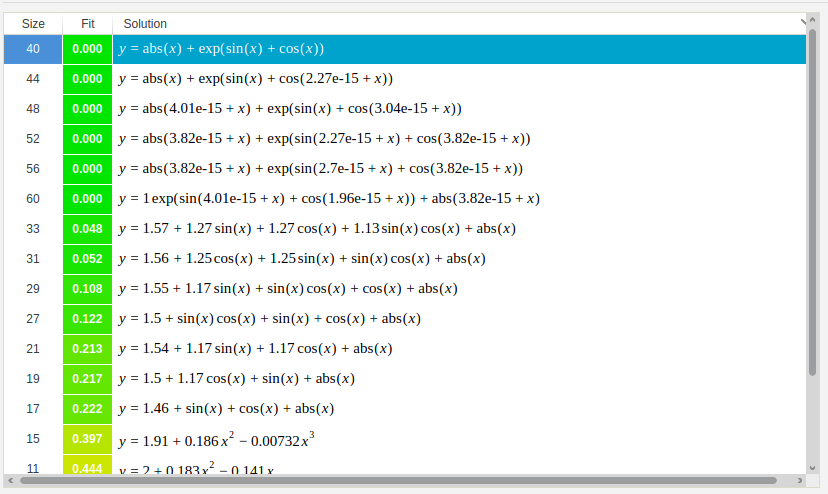
\includegraphics[width=1\linewidth]{image/solucoes_map1}
		  \caption{\centering Soluções encontradas pelo software.} 
		  \label{fig:map1_solucoes_s_ruido} 
		\end{subfigure}%
		\begin{subfigure}{.55\textwidth}
		  \centering
		  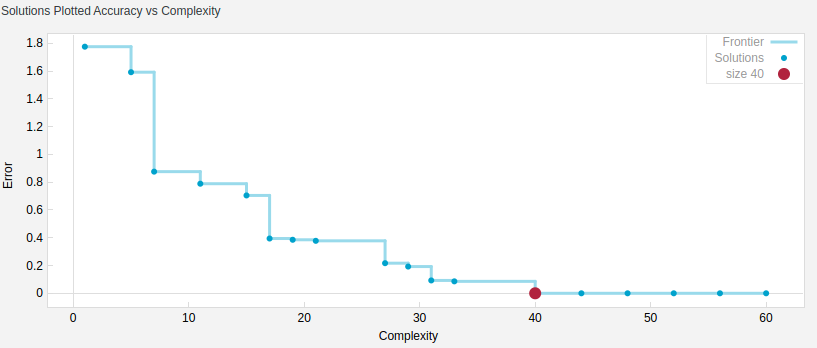
\includegraphics[width=1\linewidth]{image/pareto_map1}
		  \caption{\centering Compromisso acurácia \textit{x} simplicidade das
		  soluções.}
		  \label{fig:map1_pareto_s_ruido} 
		\end{subfigure}
	
		\begin{subfigure}{.65\textwidth}
		  \centering
		  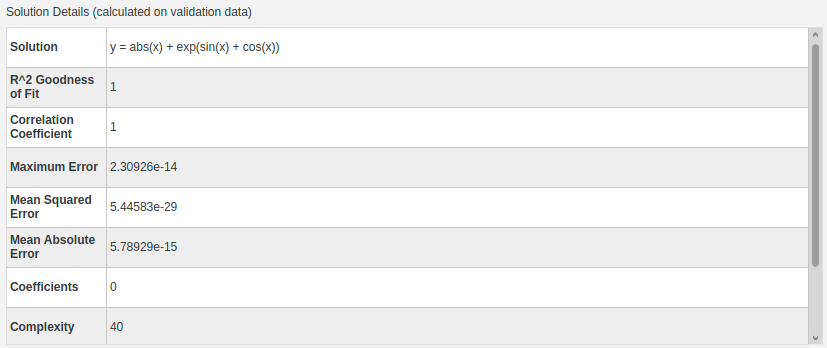
\includegraphics[width=1\linewidth]{image/best_solucao_map1}
		  \caption{\centering Resumo da melhor solução encontrada.}
		  \label{fig:map1_best_s_ruido} 
		\end{subfigure}
	
	\caption{Resultados para mapeamento da função \ref{eq:map1} sem ruídos.}
	\end{figure}
	
	\FloatBarrier

A simulação executada com os dados com ruído produziu o mapeamento representado
pela equação \ref{eq:map1_r}. A figura \ref{fig:comparaca_map1}  compara o mapeamento produzido
nesta fase com aquele utilizado para gerar os dados. Observa-se que ambos os
mapeamento estão muito próximos, porém há regiões em que as diferenças são
notáveis. Os resultados gerados pelo \textit{software} são, portanto, bastante
satisfatórios.

\begin{equation}
y = 1.61175 + 1.830094*\sin(0.792661 + x) +
0.55764*\sin(1.99325*x) + |x|
\label{eq:map1_r}
\end{equation}

\FloatBarrier
\begin{figure}[H]
		  \centering
		  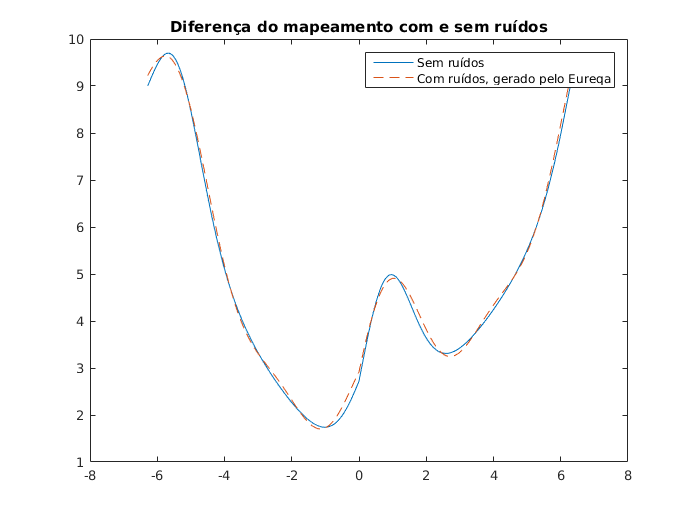
\includegraphics[width=0.65\linewidth]{image/comparacao_map1}
		  \caption{Comparação entre mapeamento com e sem ruídos.} 
		  \label{fig:comparaca_map1} 
		  
		\end{figure}
\FloatBarrier

As figuras \ref{fig:map1_solucoes_c_ruido}, \ref{fig:map1_pareto_c_ruido},
\ref{fig:map1_best_c_ruido}  e \ref{fig:map1_c_ruido} foram geradas pelo
\textit{Eureqa} e possuem informações sobre a solução encontrada. A primeira
é a lista de soluções encontradas pelo \textit{software}, a segunda mostra o
compromisso acurácia x complexidade (neste caso, a solução apresentada na
equação \ref{eq:map1_r} possui melhor compromisso, visto que seu erro é próximo
de 0 e sua complexidade, mínima), a terceira contem algumas informações sobre
a melhor solução (o erro quadrático médio neste caso é considerável,
contrariarmente ao caso sem ruído, e vale 0.625) e a última revela quais dados
foram usados para treinamento e validação, assim como o mapeamento encontrado.

\FloatBarrier
			    
	\begin{figure}[h!]
	
	\centering
	
		\begin{subfigure}{.45\textwidth} 
		  \centering
		  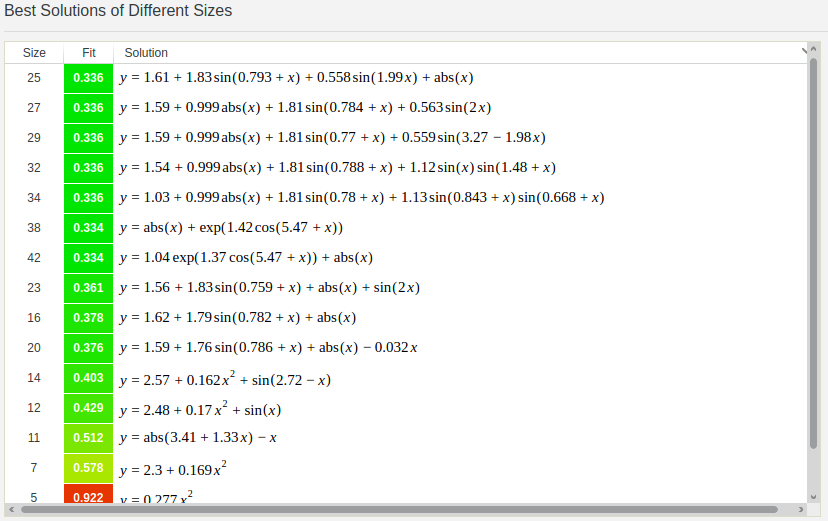
\includegraphics[width=1\linewidth]{image/best_solucao_map1_r}
		  \caption{\centering Soluções encontradas pelo software.} 
		  \label{fig:map1_solucoes_c_ruido} 
		\end{subfigure}%
		\begin{subfigure}{.55\textwidth}
		  \centering
		  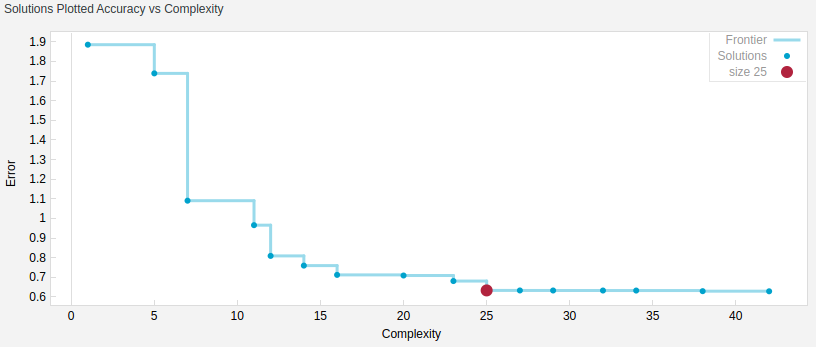
\includegraphics[width=1\linewidth]{image/pareto_map1_r}
		  \caption{\centering Compromisso acurácia \textit{x} simplicidade das
		  soluções.}
		  \label{fig:map1_pareto_c_ruido} 
		\end{subfigure}
	
		\begin{subfigure}{.5\textwidth}
		  \centering
		  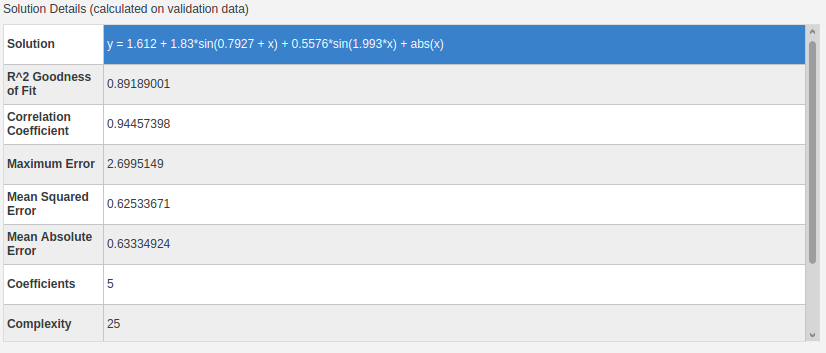
\includegraphics[width=1\linewidth]{image/best_solucao_map1_r_info}
		  \caption{\centering Resumo da melhor solução encontrada.}
		  \label{fig:map1_best_c_ruido} 
		\end{subfigure} %
		\begin{subfigure}{.45\textwidth}
		  \centering
		  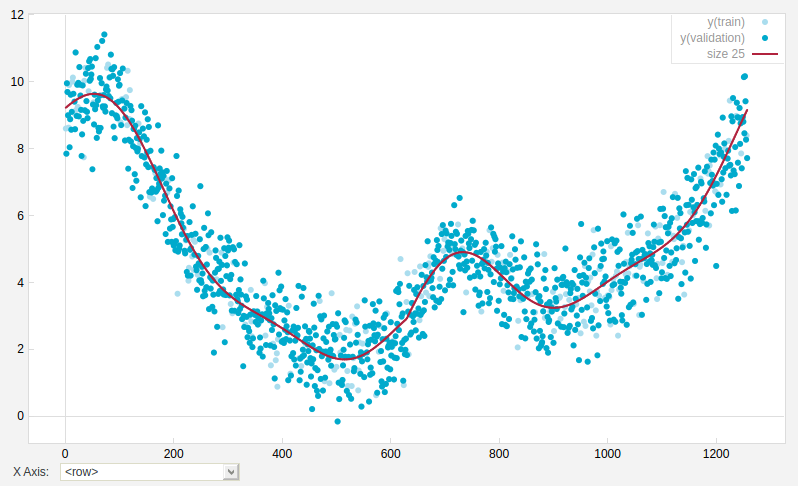
\includegraphics[width=1\linewidth]{image/solucoes_map1_r}
		  \caption{\centering Resumo do mapeamento encontrado e amostras usadas para
		  treinamento e validação.}
		  \label{fig:map1_c_ruido} 
		\end{subfigure}
	
	\caption{Resultados para mapeamento da função \ref{eq:map1} com ruídos.}
	\end{figure}
	
	\FloatBarrier

\subsection {Mapeamento y = f(x\textsubscript{1}, x\textsubscript{2},
x\textsubscript{3})}

A função escolhida para este caso está representada pela equação \ref{eq:map2},
sendo que \(x_1 \in [-3, 1]\), \(x_2 \in [1, 5]\) e \(x_3 \in [-4, 4]\). As duas
primeiras variáveis foram amostradas a cada 0.01 e a segunda, 0.02. Temos,
portanto, 401 amostras no total.

\begin{equation}
y = x_1*\log_{\pi}\left( \frac{x_2}{3}  \right) + \sqrt{2}*x_3 = 
x_1*\frac{\log_{10}\left( \frac{x_2}{3}  \right)}{\log_{10}(\pi)} + \sqrt{2}*x_3
\label{eq:map2}
\end{equation}

O mapeamento produzido pela simulação utilizando os dados sem ruídos
foi 

\begin{equation}
y =  0.959713 + 0.93436*x_3 + 0.873569*x_1*\log_{10}(x_2)
\label{eq:map2_s}
\end{equation}

O mapeamento produzido não corresponde ao utilizado para a geração dos dados,
porém os erros associados ao primeiro são praticamente nulos, isto é, o maior
erro é da ordem de \(10^{-15}\), conforme figura \ref{fig:map2_best_s_ruido}.
Isto indica que, para os os intervalos considerados para as variáveis, alguns
termos podem ser substituídos por outros sem perdas de precisão. Nota-se também,
pela figura \ref{fig:map2_solucoes_s_ruido}, que menos soluções foram encontradas em relação ao
item anterior. A imagem \ref{fig:map2_pareto_s_ruido} mostra o compromisso entre
erro e complexidade da melhor solução e é possível concluir, a partir desta
imagem, que realmente a solução de complexidade 15 supera as demais.

\FloatBarrier
			    
	\begin{figure}[h!]
	
	\centering
	
		\begin{subfigure}{.45\textwidth} 
		  \centering
		  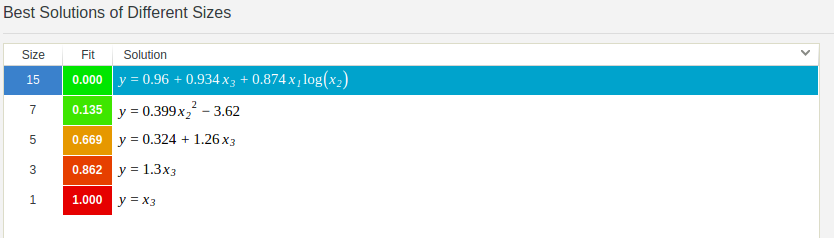
\includegraphics[width=1\linewidth]{image/solucoes_map2}
		  \caption{\centering Soluções encontradas pelo software.} 
		  \label{fig:map2_solucoes_s_ruido} 
		\end{subfigure}%
		\begin{subfigure}{.55\textwidth}
		  \centering
		  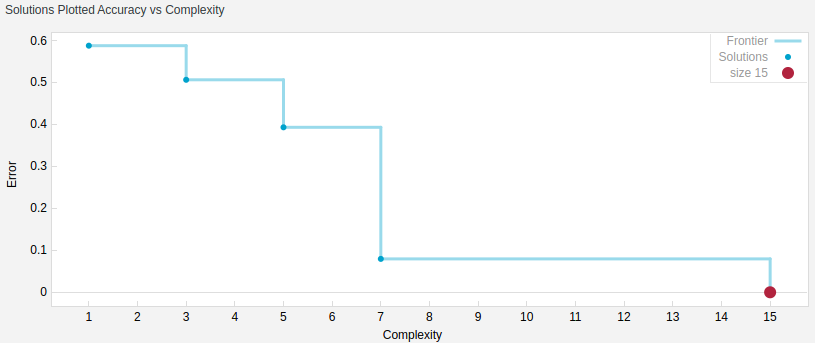
\includegraphics[width=1\linewidth]{image/pareto_map2}
		  \caption{\centering Compromisso acurácia \textit{x} simplicidade das
		  soluções.}
		  \label{fig:map2_pareto_s_ruido} 
		\end{subfigure}
	
		\begin{subfigure}{.65\textwidth}
		  \centering
		  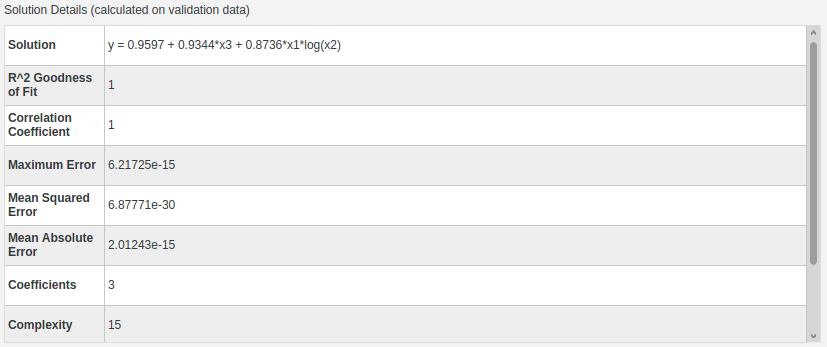
\includegraphics[width=1\linewidth]{image/best_solucao_map2_info}
		  \caption{\centering Resumo da melhor solução encontrada.}
		  \label{fig:map2_best_s_ruido} 
		\end{subfigure}
	
	\caption{Resultados para mapeamento da função \ref{eq:map2} sem ruídos.}
	\end{figure}
	
	\FloatBarrier

Enfim, a execução para os dados com ruídos gera o mapeamento 

\begin{equation}
y = 0.39025*x_2^2 - 3.555333
\label{eq:map2_r}
\end{equation}

Observa-se que \(y\) não depende de \(x_1\) e \(x_3\) neste caso. As figuras a
seguir foram geradas pelo \textit{software}. Destacam-se os seguintes fatos:

\begin{itemize}
  \item A figura \ref{fig:map2_pareto_c_ruido} mostra o compromisso entre erro e
  complexidade para as melhores soluções. Nota-se que, apesar de a solução não
  apresentar o menor erro, ela possui uma maior simplicidade comparada às
  demais. Sendo assim, ela é escolhida como a melhor solução atendendo aos
  critérios de acurácia e complexidade simultaneamente.
  \item Conforme figura \ref{fig:map2_best_c_ruido}, o erro quadrático médio é
  considerável e vale, aproximadamente, 0.70.
  \item A figura \ref{fig:map2_c_ruido} representa o mapeamento e as amostras
  utilizadas. Observa-se que este mapeamento aproxima-se relativamente bem aos
  dados.
\end{itemize}

\FloatBarrier
			    
	\begin{figure}[h!]
	
	\centering
	
		\begin{subfigure}{.45\textwidth} 
		  \centering
		  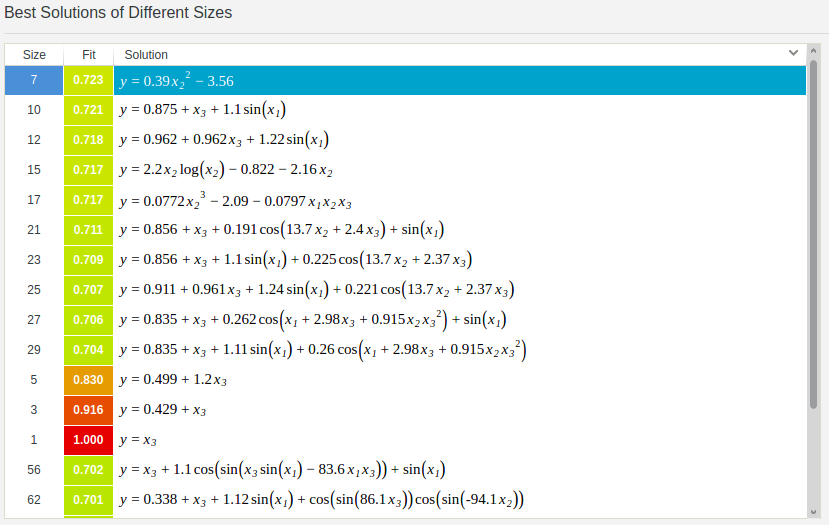
\includegraphics[width=1\linewidth]{image/solucoes_map2_r}
		  \caption{\centering Soluções encontradas pelo software.} 
		  \label{fig:map2_solucoes_c_ruido} 
		\end{subfigure}%
		\begin{subfigure}{.55\textwidth}
		  \centering
		  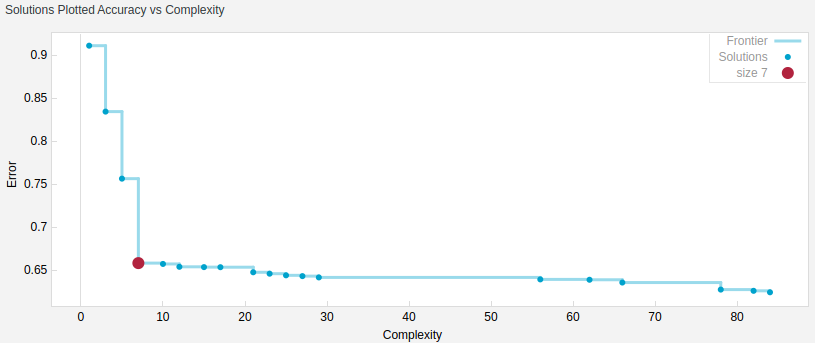
\includegraphics[width=1\linewidth]{image/pareto_map2_r}
		  \caption{\centering Compromisso acurácia \textit{x} simplicidade das
		  soluções.}
		  \label{fig:map2_pareto_c_ruido} 
		\end{subfigure}
	
		\begin{subfigure}{.5\textwidth}
		  \centering
		  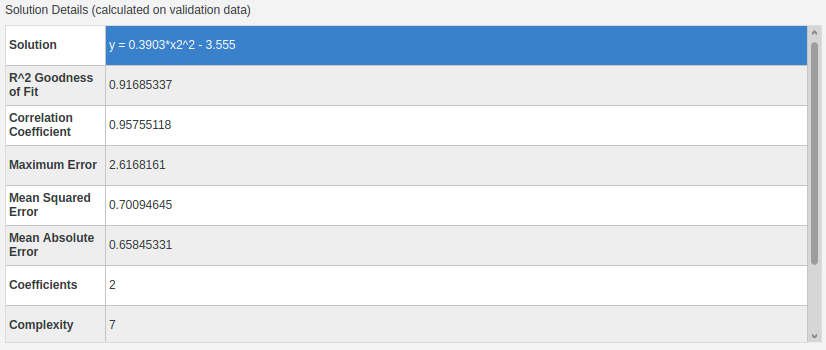
\includegraphics[width=1\linewidth]{image/best_solucao_map2_r_info}
		  \caption{\centering Resumo da melhor solução encontrada.}
		  \label{fig:map2_best_c_ruido} 
		\end{subfigure} %
		\begin{subfigure}{.45\textwidth}
		  \centering
		  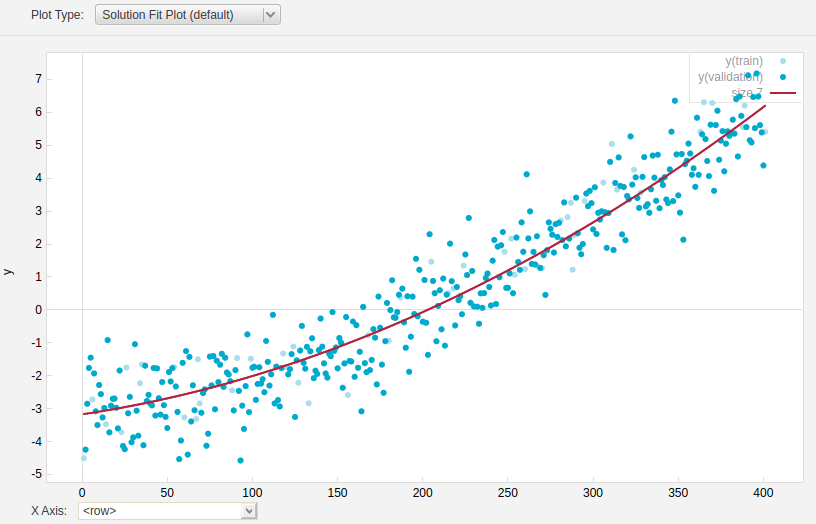
\includegraphics[width=1\linewidth]{image/best_solucao_map2_r}
		  \caption{\centering Resumo do mapeamento encontrado e amostras usadas para
		  treinamento e validação.}
		  \label{fig:map2_c_ruido} 
		\end{subfigure}
	
	\caption{Resultados para mapeamento da função \ref{eq:map2} com ruídos.}
	\end{figure}
	
	\FloatBarrier 
